
Fitting and plotting various trends

\begin{lstlisting}
# time plot of U.S. GNP and various fitted trends
par(mfrow=c(2,2))
par(oma=c(0,2,4,2))

# global quadratic trend
plot(x=1947.25+gnp.t,y=gnp.v,type="b",ylim=c(200,800),xlab="time",ylab="U.S. GNP",main="Global quadratic trend",col="green4")
lines(1947.25+gnp.t,predict(object=gqt.lm),col="blue")
legend(x="topleft",legend=c("actual values","estimated global trend"),col=c("green4","blue","red"),lty=c(1,1),pch=c(1,-1))

# global cubic trend
plot(x=1947.25+gnp.t,y=gnp.v,type="b",ylim=c(200,800),xlab="time",ylab="U.S. GNP",main="Global cubic trend",col="green4")
lines(1947.25+gnp.t,predict(object=gct.lm),col="blue")

# global multiplicative exponential trend
plot(x=1947.25+gnp.t,y=gnp.v,type="b",ylim=c(200,800),xlab="time",ylab="U.S. GNP",main="Global multiplicative exponential trend",col="green4")
lines(1947.25+gnp.t,exp(predict(object=gmet.lm)),col="blue")

# global additive exponential trend
plot(x=1947.25+gnp.t,y=gnp.v,type="b",ylim=c(200,800),xlab="time",ylab="U.S. GNP",main="Global additive exponential trend",col="green4")
lines(1947.25+gnp.t,predict(object=gaet.nls),col="blue")

mtext(text="Time plots of U.S. GNP and fitted trends",side=3,line=0,outer=T)
\end{lstlisting}

\begin{figure}[H]
\centering
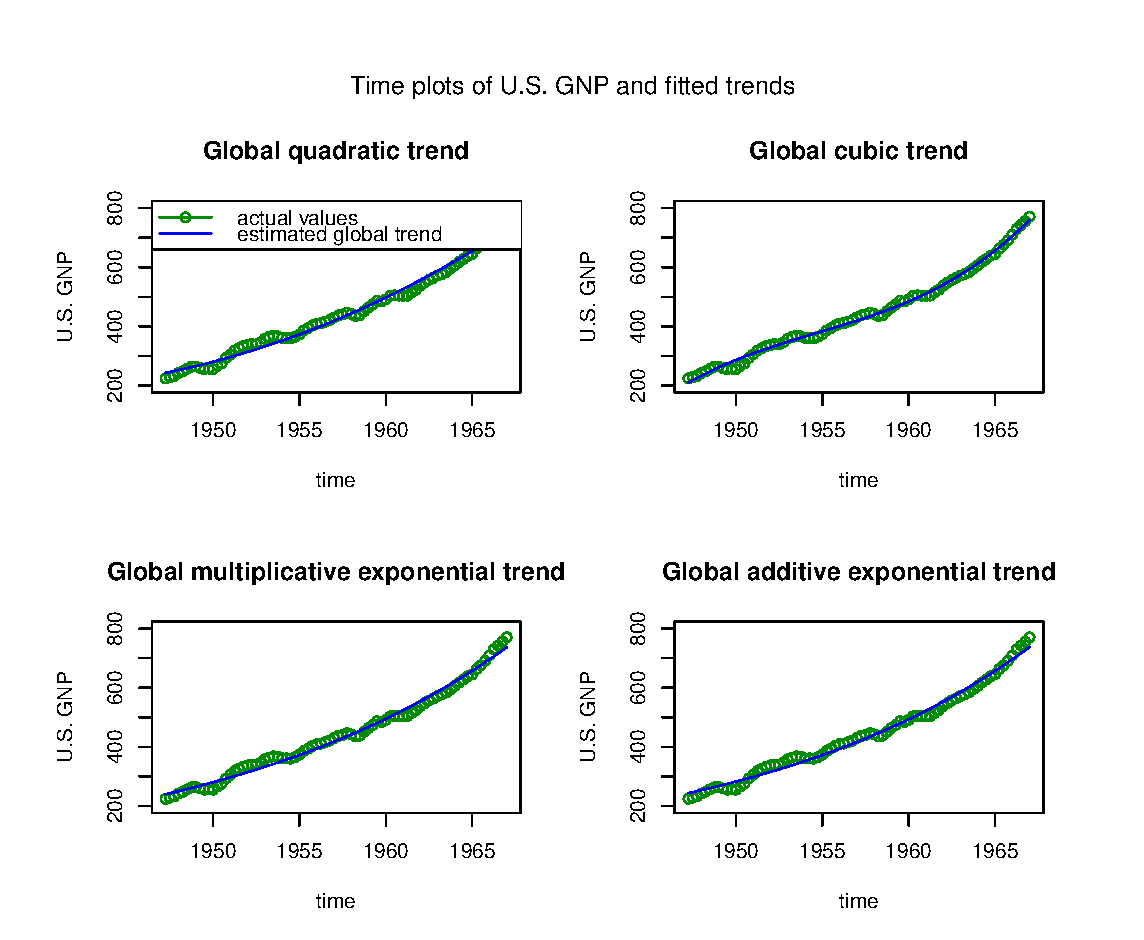
\includegraphics[width=0.8\textwidth]{plots/Rplot1.pdf}
\caption{Various Fits}
\end{figure}

\subsection{Analysis of Precipitation and Temperature Data in Zurich}

We begin our analysis by looking at the raw series and a deseasonalized series for the precipitation data:

\begin{lstlisting}
# define variables
  sf=1
  raw.data.ex.season <- deseason(raw.data)
  raw.data.ex.trend.KS <- detrend(raw.data,ma=F,sf)
  raw.data.ex.trend.KS.ex.season <- deseason(raw.data.ex.trend.KS$detrended.series)
  
# define axis labels
  acf.x.lab <- expression(paste("lag ",tau,sep=""))
  acf.y.lab <- expression(paste("acf(",tau,")",sep=""))

# time plot and correlogram of deseasonalized data 
  par(mfrow=c(2,2))
  par(oma=c(0,2,4,2))
  plot(x=raw.data,type="b",xlab="Time",ylab=ylabel,main="Raw series",col=line.color)
  plot(x=raw.data.ex.season$deseasoned.series,type="b",xlab="Time",ylab=ylabel,main="Deseasonalized series",col=line.color)
  acf(x=raw.data,xlab=acf.x.lab,ylab=acf.y.lab,main="")
  acf(x=raw.data.ex.season$deseasoned.series,xlab=acf.x.lab,ylab=acf.y.lab,main="")
  mtext(text=title.text,side=3,line=0,outer=T)
\end{lstlisting}

\begin{figure}[H]
\centering
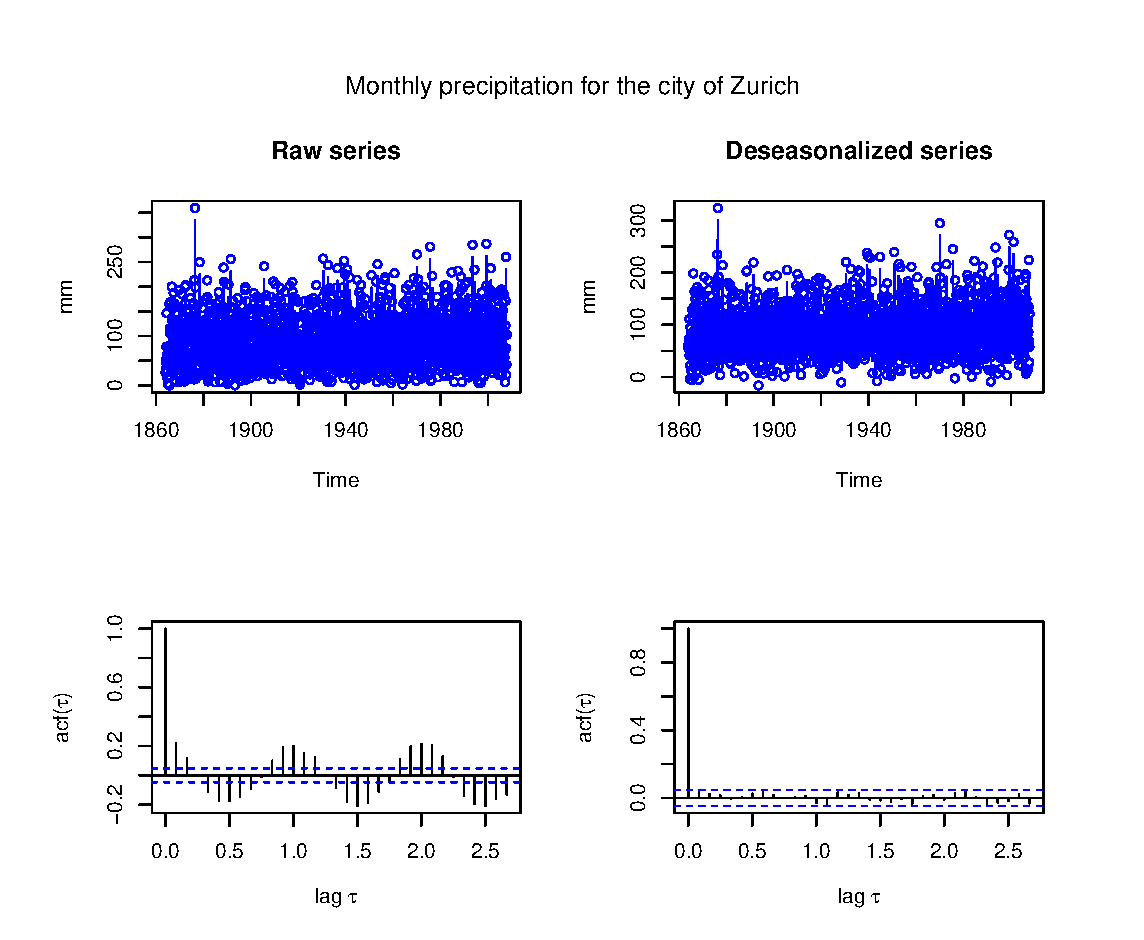
\includegraphics[width=0.8\textwidth]{plots/ZHP1.pdf}
\caption{Precipitation}
\end{figure}

The correlogram for the raw series shows that there is a lot of significant correlation at almost all lags and there is a clear seasonal pattern to it. Whereas the deseasonalized correlogram makes the series appear stationary. \\

To confirm that there is a seasonal effect we look at this effect on its own: 

\begin{lstlisting}
# plot of seasonal effects [ZHP2]
  par(mfrow=c(1,1))
  par(oma=c(0,2,4,2))
  plot(raw.data.ex.season$season.effects,type="b",col=line.color,xlab="Month",ylab="Effect",main="Seasonal effects")
\end{lstlisting}


\begin{figure}[H]
\centering
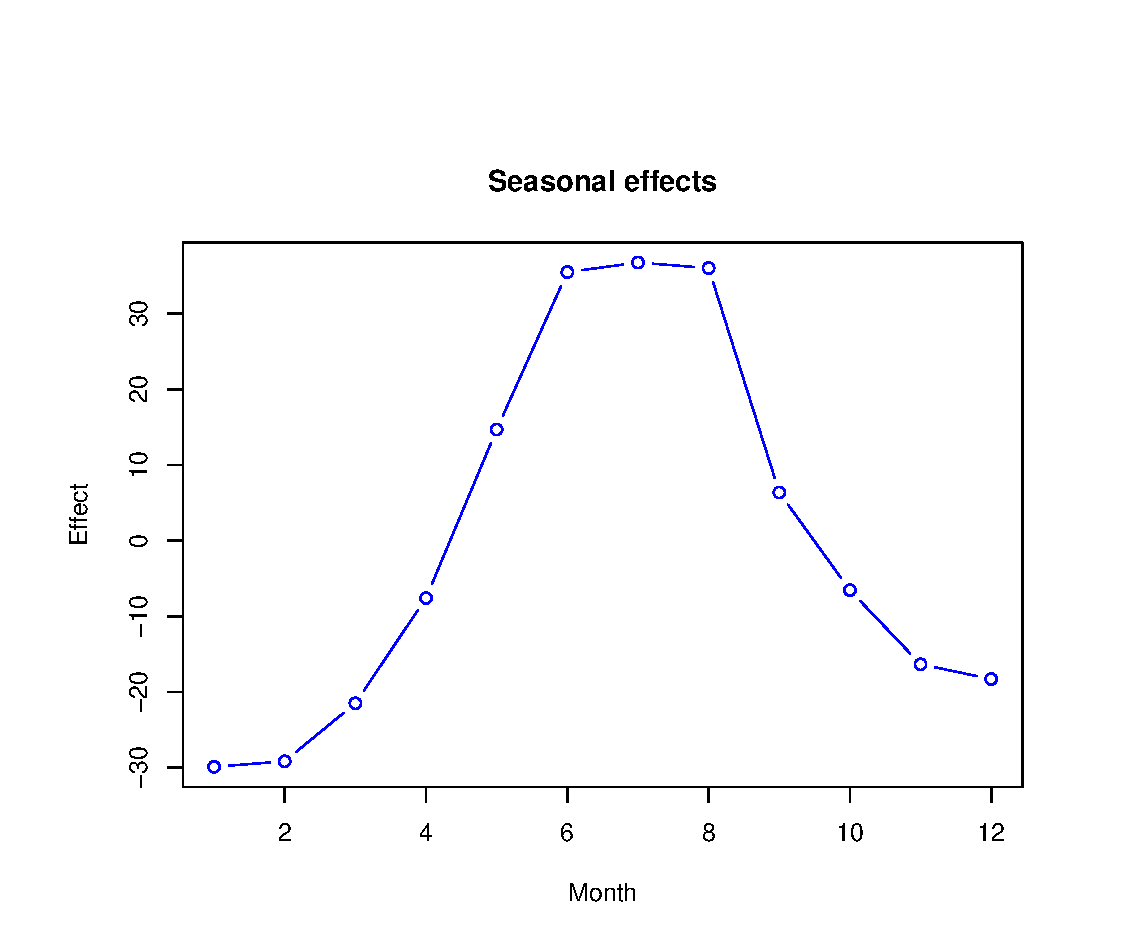
\includegraphics[width=0.6\textwidth]{plots/ZHP2.pdf}
\caption{Seasonal effects}
\end{figure}

When we look at the temperature data, we can observe that there is a linear trend in the raw series. But as the middle graph shows differencing alone does not make the series stationary, we again need to deseasonalize it.

\begin{lstlisting}
# time plots and correlograms of deseasonalized KS-detrended data
  par(mfrow=c(2,3))
  par(oma=c(0,2,4,2))
  plot(x=raw.data,type="b",xlab="time",ylab=ylabel,main="raw series",col=line.color)
  lines(x=as.numeric(time(raw.data.ex.trend.KS$trend)),y=as.numeric(raw.data.ex.trend.KS$trend),col="red")
  plot(x=raw.data.ex.trend.KS$detrended.series,type="b",xlab="Time",ylab=ylabel,main="KS-detrended series",col=line.color)
  plot(x=raw.data.ex.trend.KS.ex.season$deseasoned.series,type="b",xlab="time",ylab=ylabel,main="deseasonalized KS-detrended series",col=line.color)
  acf(x=raw.data,xlab=acf.x.lab,ylab=acf.y.lab,main="")
  acf(x=raw.data.ex.trend.KS$detrended.series,xlab=acf.x.lab,ylab=acf.y.lab,main="")
  acf(x=raw.data.ex.trend.KS.ex.season$deseasoned.series,xlab=acf.x.lab,ylab=acf.y.lab,main="")
  mtext(text=paste(title.text," (KS-detrended)",sep=""),side=3,line=0,outer=T)
\end{lstlisting}

\begin{figure}[H]
\centering
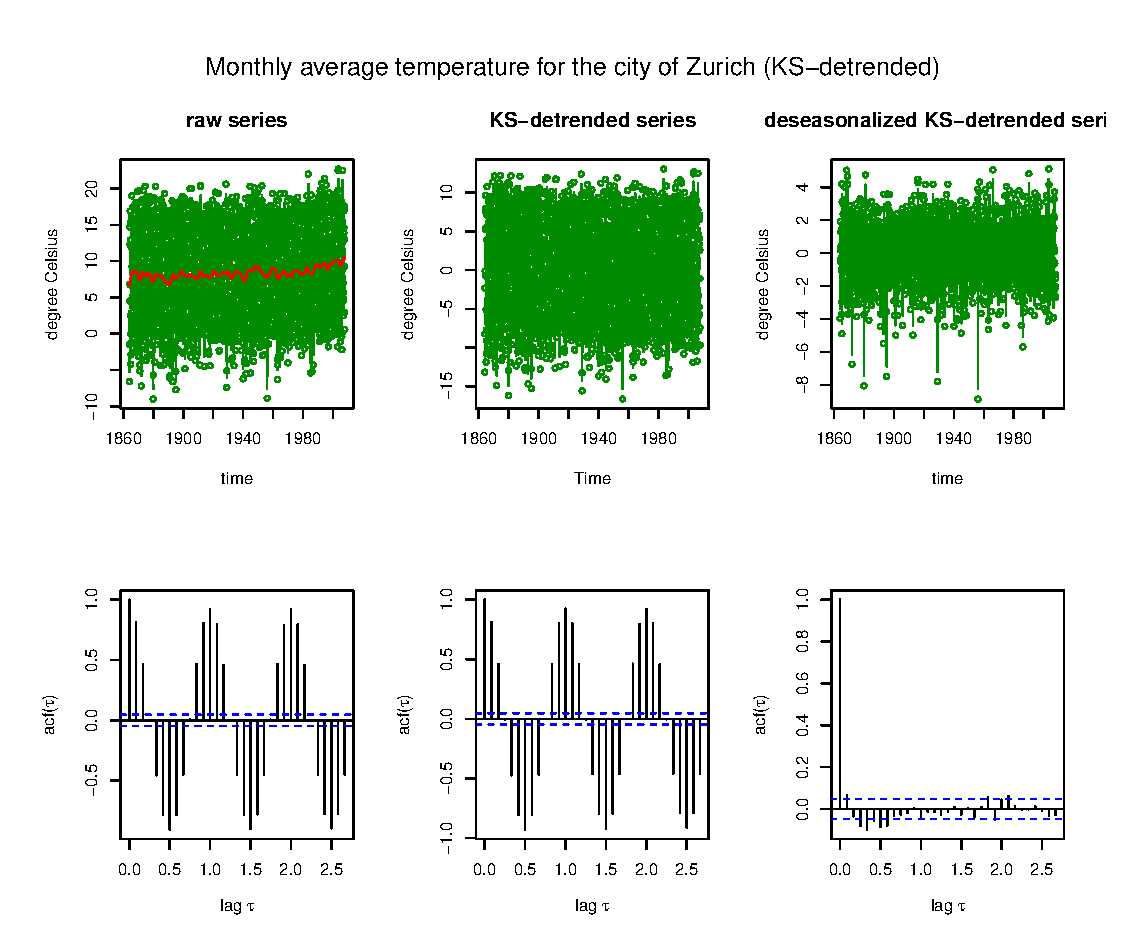
\includegraphics[width=0.8\textwidth]{plots/ZHP4.pdf}
\caption{Temperature}
\end{figure}

\subsection{Unemployment Data}

We see looking at the raw data, the trend line and the correlogram, that there is significant correlation at all lags. After detrending the correlogram shows that the trend is somewhat dissappeared, but there is still seasonality.

\begin{figure}[H]
\centering
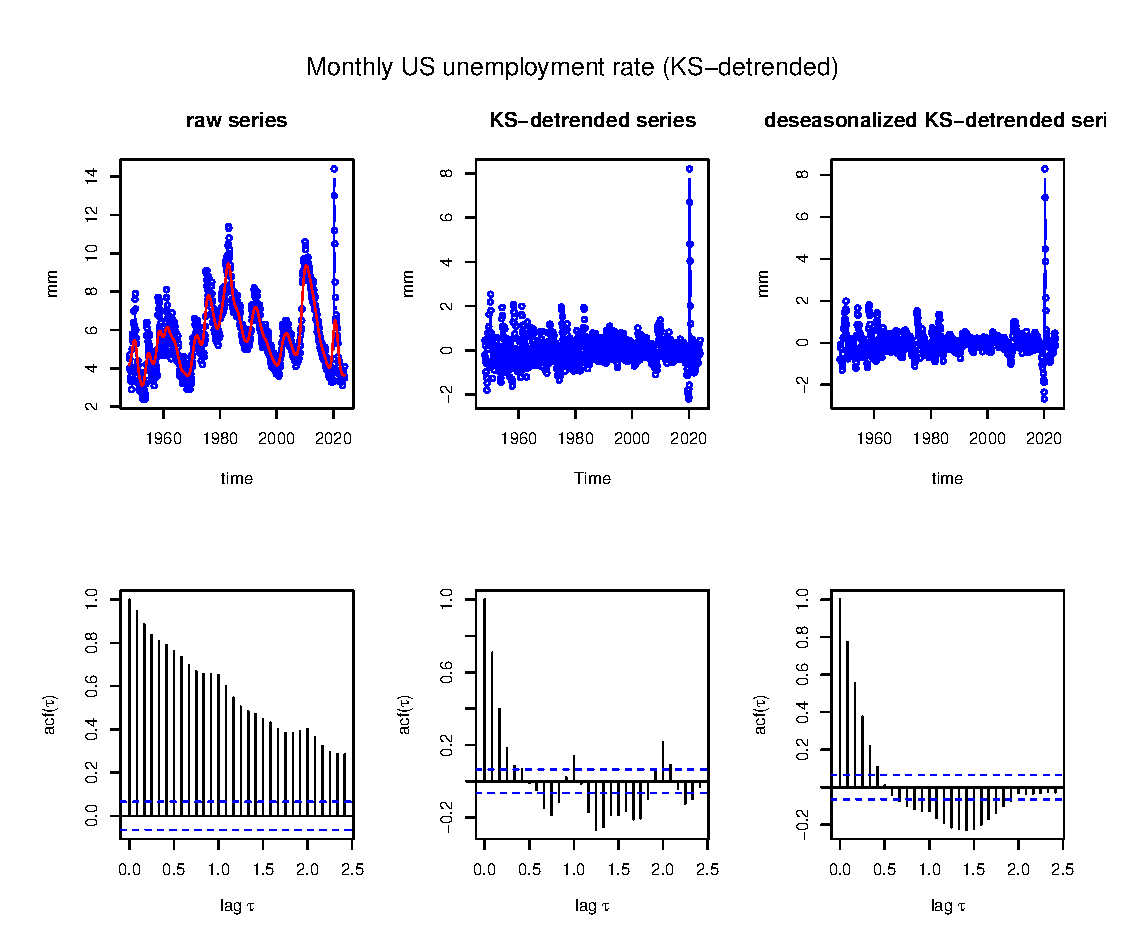
\includegraphics[width=0.8\textwidth]{plots/UEMP.pdf}
\caption{Unemployment}
\end{figure}


\subsection{Stock data}

\begin{lstlisting}
stock <- read.csv('/Users/michaelsigg/Desktop/Master/FS24/Time Series Analysis/Exc. 3/NVDA.csv', sep=',') # https://finance.yahoo.com/quote/NVDA/history?period1=916963200&period2=1709856000&interval=1d&filter=history&frequency=1d&includeAdjustedClose=true
stock$Date <- as.Date(stock$Date, "%Y-%m-%d")
stock$LogClose = log(stock$Close)

stock$DeltaClose = c(NA, diff(stock$Close))

stock$LogClose = log(stock$Close)
stock$DeltaLogClose = c(NA, diff(stock$LogClose))

par(mfrow=c(2,2))
par(oma=c(0,2,4,2))
plot(stock$Date, stock$Close, type = 'l', xlab = "Time", ylab = "Close Price", main = 'Close Price')
plot(stock$Date, stock$LogClose, type = 'l', xlab = "Time", ylab = "Log Close Price", main = 'Log(Close Price)')
plot(stock$Date, stock$DeltaClose, type = 'l', xlab = "Time", ylab = "Delta Close Price", main = 'Differenced Close Price')
plot(stock$Date, stock$DeltaLogClose, type = 'l', xlab = "Time", ylab = "Delta Log Close Price", main = 'Differenced Log(Close Price)')
mtext(text="NVIDIA historical price charts",side=3,line=0,outer=T)
\end{lstlisting}

\begin{figure}[H]
\centering
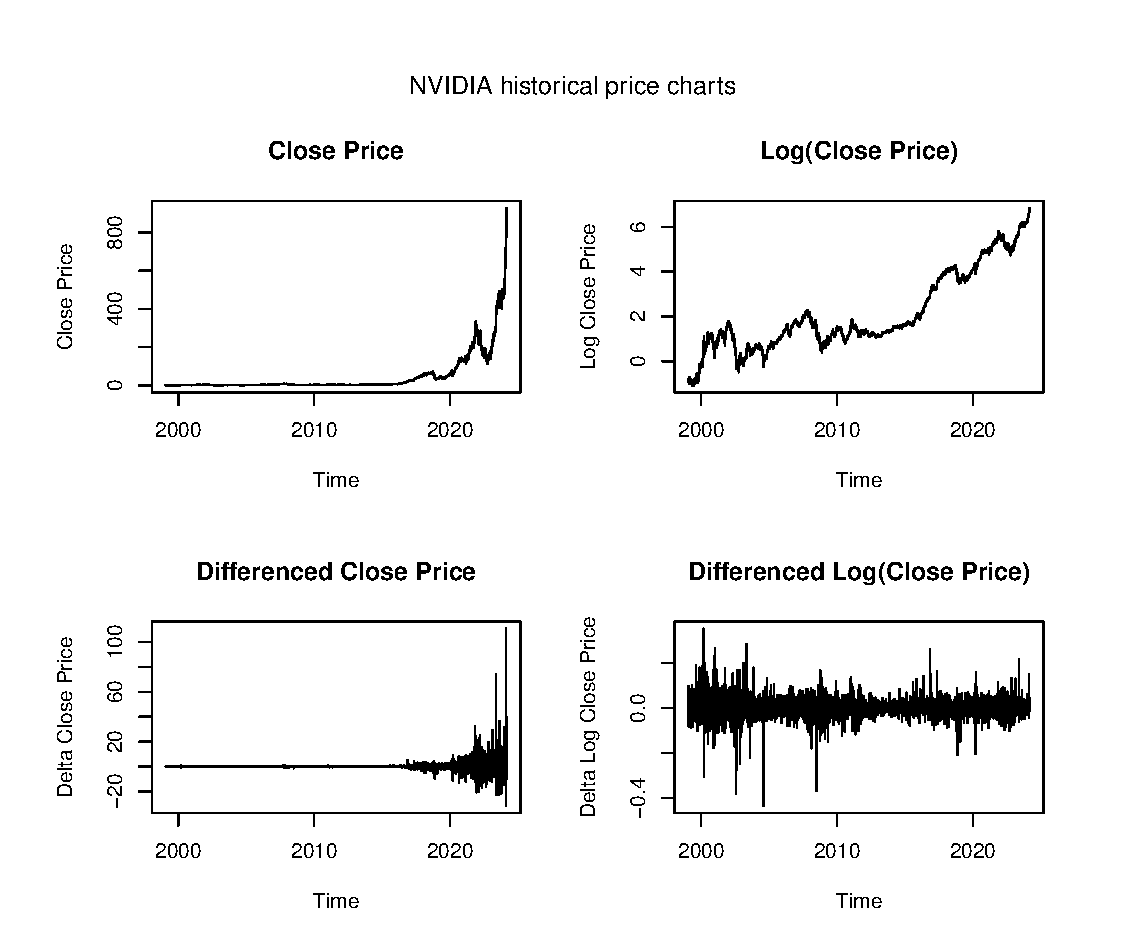
\includegraphics[width=0.8\textwidth]{plots/NVD.pdf}
\caption{NVIDIA Price Charts}
\end{figure}

Already at first look, it is clear that differencing the data is not enough to make it stationary. Lets look at the autocorrelation and partial autocorrelation function:

\begin{lstlisting}
stock.acf <- acf(na.omit(stock$DeltaClose), lag.max = 100, main = "Delta Close Price")
stock.pacf <- pacf(na.omit(stock$DeltaClose), lag.max = 100, main = "Delta Close Price")

logstock.acf <- acf(na.omit(stock$DeltaLogClose), lag.max = 100, main = "Delta Log Close Price")
logstock.pacf <- pacf(na.omit(stock$DeltaLogClose), lag.max = 100, main = "Delta Log Close Price")
\end{lstlisting}

\begin{figure}[H]
\centering
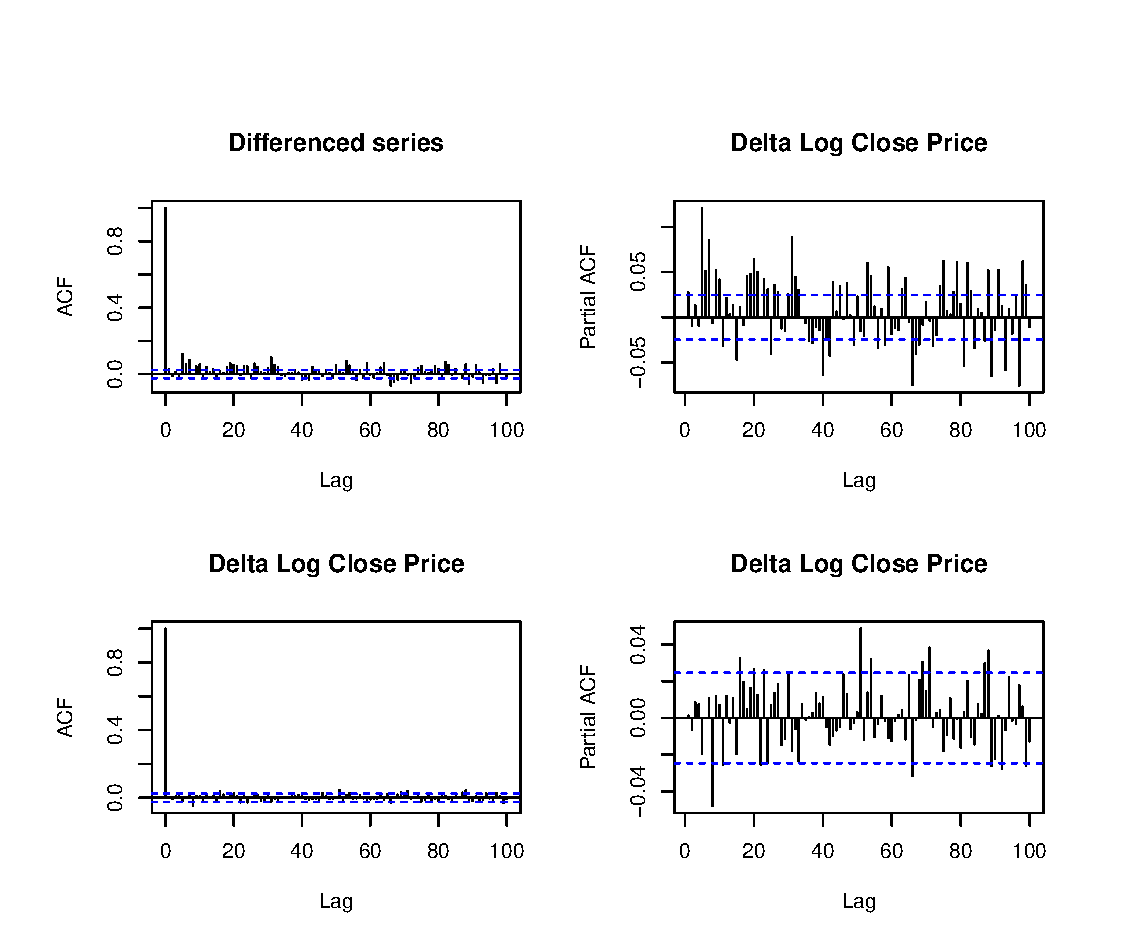
\includegraphics[width=0.8\textwidth]{plots/NVD2.pdf}
\caption{NVIDIA Correlograms}
\end{figure}

We see here that both the acf and the pacf for the differenced data indicates non-stationarity. Taking the log addresses this issue. (Note that the lags that still have significant correlation are expected to appear just by chance. As we have a 95\% CI, out of 100 lags we'd expect around 10 to have significant correlation just by chance). 

\begin{lstlisting}
fit.diff <- arima(stock$DeltaClose, c(0,0,0))
fit.diff
tsdiag(fit.diff)

\end{lstlisting}

\begin{figure}[H]
\centering
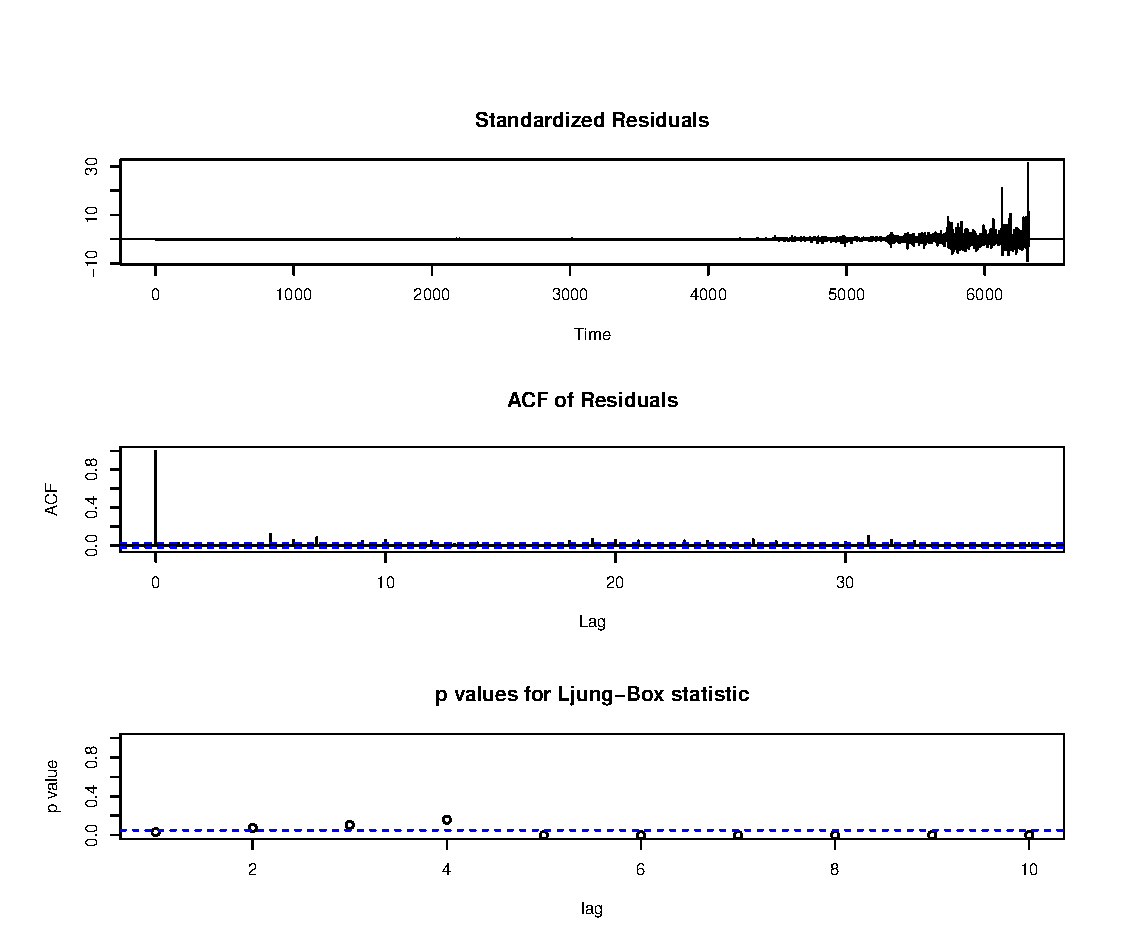
\includegraphics[width=0.8\textwidth]{plots/NVD3.pdf}
\caption{Differenced Closing Price}
\end{figure}

This shows that when we fit an ARMA(0,0,0) model (i.e., a white noise process) the residuals still shows significant correlation at various lags. And the Ljung-Box Statistic confirms that we can reject the null hypothesis of no autocorrelation for several lag intervals, it confirms that the residuals are not white noise. 

\begin{lstlisting}
fit.diff.log <- arima(stock$DeltaLogClose, c(0,0,0))
fit.diff.log
tsdiag(fit.diff.log)
\end{lstlisting}

\begin{figure}[H]
\centering
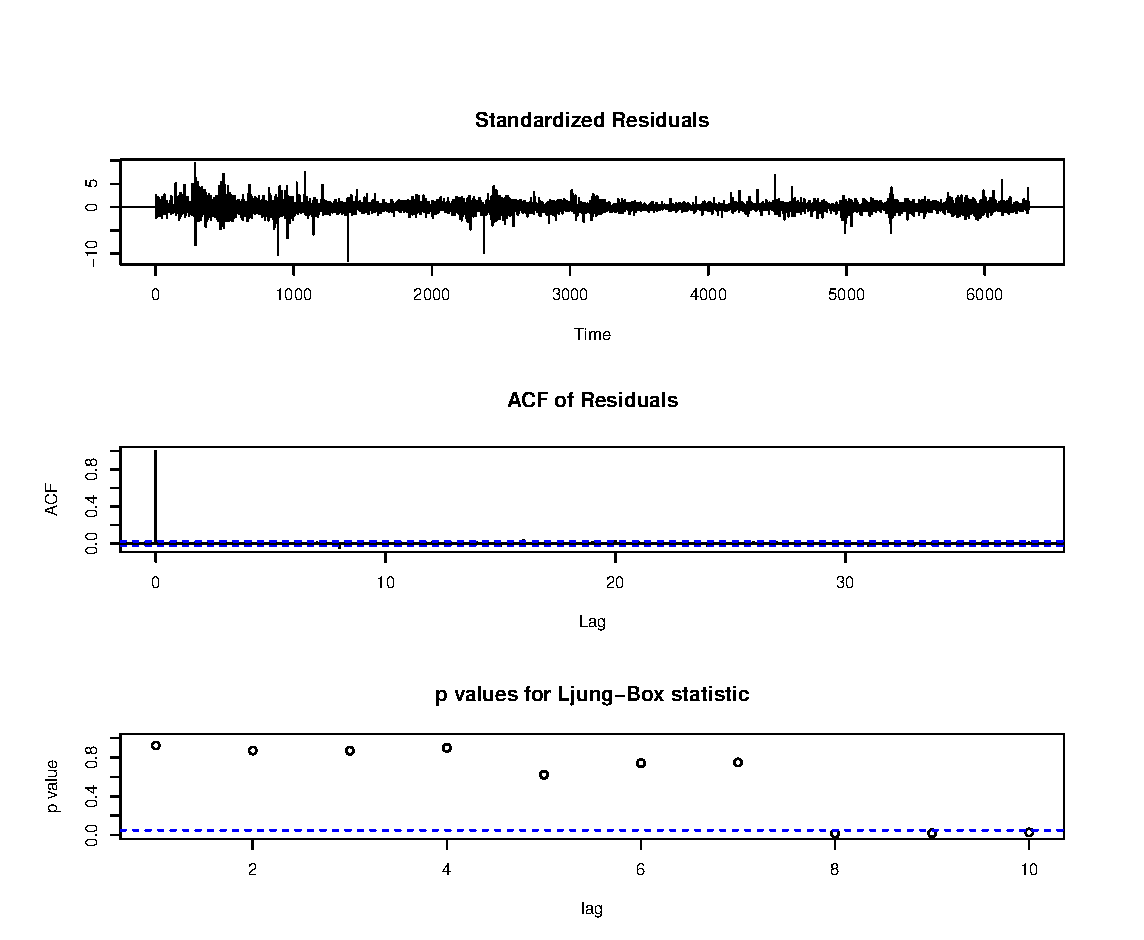
\includegraphics[width=0.8\textwidth]{plots/NVD4.pdf}
\caption{Differenced Log Closing Price }
\end{figure}

 When we fit the same ARMA(0,0,0) model to the log data, we can see that the residuals show no signs of autocorrelation and we can not reject the null hypothesis of the Ljung-Box Test, that the residuals are not white noise. 